

\tikzset{every picture/.style={line width=0.75pt}} %set default line width to 0.75pt        

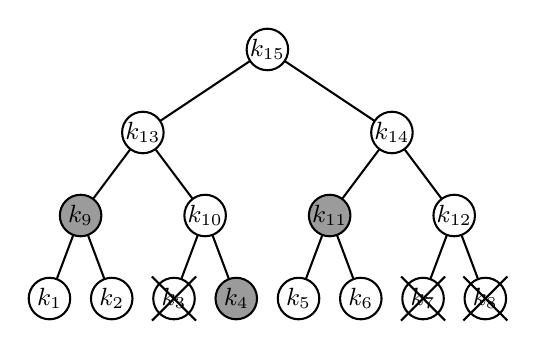
\begin{tikzpicture}[x=0.75pt,y=0.75pt,yscale=-1,xscale=1]
%uncomment if require: \path (0,156); %set diagram left start at 0, and has height of 156

%Straight Lines [id:da7264618821071116] 
\draw    (25,90) -- (10,130) ;
%Straight Lines [id:da021214228424441206] 
\draw    (25,90) -- (40,130) ;
%Straight Lines [id:da7682983898858589] 
\draw    (85,90) -- (70,130) ;
%Straight Lines [id:da680770082896881] 
\draw    (85,90) -- (100,130) ;
%Straight Lines [id:da801506955071976] 
\draw    (145,90) -- (130,130) ;
%Straight Lines [id:da043152738546742064] 
\draw [line width=0.75]    (145,90) -- (160,130) ;
%Straight Lines [id:da8853377273892189] 
\draw    (205,90) -- (190,130) ;
%Straight Lines [id:da7252869978645777] 
\draw    (205,90) -- (220,130) ;
%Straight Lines [id:da02572385855624737] 
\draw    (55,50) -- (25,90) ;
%Straight Lines [id:da30458044388997774] 
\draw    (55,50) -- (85,90) ;
%Straight Lines [id:da17661087510957563] 
\draw [line width=0.75]    (175,50) -- (145,90) ;
%Straight Lines [id:da6362344930800443] 
\draw    (175,50) -- (205,90) ;
%Straight Lines [id:da9010420336797604] 
\draw    (115,10) -- (55,50) ;
%Straight Lines [id:da9254861663329741] 
\draw [line width=0.75]    (115,10) -- (175,50) ;
%Shape: Circle [id:dp5148351832942917] 
\draw  [fill={rgb, 255:red, 255; green, 255; blue, 255 }  ,fill opacity=1 ][line width=0.75]  (0,130) .. controls (0,124.48) and (4.48,120) .. (10,120) .. controls (15.52,120) and (20,124.48) .. (20,130) .. controls (20,135.52) and (15.52,140) .. (10,140) .. controls (4.48,140) and (0,135.52) .. (0,130) -- cycle ;
%Shape: Circle [id:dp8202362949298456] 
\draw  [fill={rgb, 255:red, 255; green, 255; blue, 255 }  ,fill opacity=1 ][line width=0.75]  (30,130) .. controls (30,124.48) and (34.48,120) .. (40,120) .. controls (45.52,120) and (50,124.48) .. (50,130) .. controls (50,135.52) and (45.52,140) .. (40,140) .. controls (34.48,140) and (30,135.52) .. (30,130) -- cycle ;
%Shape: Circle [id:dp29796828256931085] 
\draw  [fill={rgb, 255:red, 255; green, 255; blue, 255 }  ,fill opacity=1 ][line width=0.75]  (60,130) .. controls (60,124.48) and (64.48,120) .. (70,120) .. controls (75.52,120) and (80,124.48) .. (80,130) .. controls (80,135.52) and (75.52,140) .. (70,140) .. controls (64.48,140) and (60,135.52) .. (60,130) -- cycle ;
%Shape: Circle [id:dp27916620429373196] 
\draw  [fill={rgb, 255:red, 155; green, 155; blue, 155 }  ,fill opacity=1 ][line width=0.75]  (90,130) .. controls (90,124.48) and (94.48,120) .. (100,120) .. controls (105.52,120) and (110,124.48) .. (110,130) .. controls (110,135.52) and (105.52,140) .. (100,140) .. controls (94.48,140) and (90,135.52) .. (90,130) -- cycle ;
%Shape: Circle [id:dp29565933370139774] 
\draw  [fill={rgb, 255:red, 255; green, 255; blue, 255 }  ,fill opacity=1 ][line width=0.75]  (120,130) .. controls (120,124.48) and (124.48,120) .. (130,120) .. controls (135.52,120) and (140,124.48) .. (140,130) .. controls (140,135.52) and (135.52,140) .. (130,140) .. controls (124.48,140) and (120,135.52) .. (120,130) -- cycle ;
%Shape: Circle [id:dp025397782343626663] 
\draw  [fill={rgb, 255:red, 255; green, 255; blue, 255 }  ,fill opacity=1 ][line width=0.75]  (150,130) .. controls (150,124.48) and (154.48,120) .. (160,120) .. controls (165.52,120) and (170,124.48) .. (170,130) .. controls (170,135.52) and (165.52,140) .. (160,140) .. controls (154.48,140) and (150,135.52) .. (150,130) -- cycle ;
%Shape: Circle [id:dp653970469885407] 
\draw  [fill={rgb, 255:red, 255; green, 255; blue, 255 }  ,fill opacity=1 ][line width=0.75]  (180,130) .. controls (180,124.48) and (184.48,120) .. (190,120) .. controls (195.52,120) and (200,124.48) .. (200,130) .. controls (200,135.52) and (195.52,140) .. (190,140) .. controls (184.48,140) and (180,135.52) .. (180,130) -- cycle ;
%Shape: Circle [id:dp2542641018476448] 
\draw  [fill={rgb, 255:red, 255; green, 255; blue, 255 }  ,fill opacity=1 ][line width=0.75]  (210,130) .. controls (210,124.48) and (214.48,120) .. (220,120) .. controls (225.52,120) and (230,124.48) .. (230,130) .. controls (230,135.52) and (225.52,140) .. (220,140) .. controls (214.48,140) and (210,135.52) .. (210,130) -- cycle ;
%Shape: Circle [id:dp7410189340861388] 
\draw  [fill={rgb, 255:red, 155; green, 155; blue, 155 }  ,fill opacity=1 ][line width=0.75]  (15,90) .. controls (15,84.48) and (19.48,80) .. (25,80) .. controls (30.52,80) and (35,84.48) .. (35,90) .. controls (35,95.52) and (30.52,100) .. (25,100) .. controls (19.48,100) and (15,95.52) .. (15,90) -- cycle ;
%Shape: Circle [id:dp11686287881251745] 
\draw  [fill={rgb, 255:red, 255; green, 255; blue, 255 }  ,fill opacity=1 ][line width=0.75]  (75,90) .. controls (75,84.48) and (79.48,80) .. (85,80) .. controls (90.52,80) and (95,84.48) .. (95,90) .. controls (95,95.52) and (90.52,100) .. (85,100) .. controls (79.48,100) and (75,95.52) .. (75,90) -- cycle ;
%Shape: Circle [id:dp9012744756772677] 
\draw  [fill={rgb, 255:red, 155; green, 155; blue, 155 }  ,fill opacity=1 ][line width=0.75]  (135,90) .. controls (135,84.48) and (139.48,80) .. (145,80) .. controls (150.52,80) and (155,84.48) .. (155,90) .. controls (155,95.52) and (150.52,100) .. (145,100) .. controls (139.48,100) and (135,95.52) .. (135,90) -- cycle ;
%Shape: Circle [id:dp24117777074385538] 
\draw  [fill={rgb, 255:red, 255; green, 255; blue, 255 }  ,fill opacity=1 ][line width=0.75]  (195,90) .. controls (195,84.48) and (199.48,80) .. (205,80) .. controls (210.52,80) and (215,84.48) .. (215,90) .. controls (215,95.52) and (210.52,100) .. (205,100) .. controls (199.48,100) and (195,95.52) .. (195,90) -- cycle ;
%Shape: Circle [id:dp3084697229561302] 
\draw  [fill={rgb, 255:red, 255; green, 255; blue, 255 }  ,fill opacity=1 ][line width=0.75]  (45,50) .. controls (45,44.48) and (49.48,40) .. (55,40) .. controls (60.52,40) and (65,44.48) .. (65,50) .. controls (65,55.52) and (60.52,60) .. (55,60) .. controls (49.48,60) and (45,55.52) .. (45,50) -- cycle ;
%Shape: Circle [id:dp3751790613196788] 
\draw  [fill={rgb, 255:red, 255; green, 255; blue, 255 }  ,fill opacity=1 ][line width=0.75]  (165,50) .. controls (165,44.48) and (169.48,40) .. (175,40) .. controls (180.52,40) and (185,44.48) .. (185,50) .. controls (185,55.52) and (180.52,60) .. (175,60) .. controls (169.48,60) and (165,55.52) .. (165,50) -- cycle ;
%Shape: Circle [id:dp9802416358387074] 
\draw  [fill={rgb, 255:red, 255; green, 255; blue, 255 }  ,fill opacity=1 ][line width=0.75]  (105,10) .. controls (105,4.48) and (109.48,0) .. (115,0) .. controls (120.52,0) and (125,4.48) .. (125,10) .. controls (125,15.52) and (120.52,20) .. (115,20) .. controls (109.48,20) and (105,15.52) .. (105,10) -- cycle ;
\draw   (59.39,119.39) -- (80.61,140.61)(80.61,119.39) -- (59.39,140.61) ;
\draw   (179.39,119.39) -- (200.61,140.61)(200.61,119.39) -- (179.39,140.61) ;
\draw   (209.39,119.39) -- (230.61,140.61)(230.61,119.39) -- (209.39,140.61) ;

% Text Node
\draw (115,10) node  [font=\small]  {$k_{15}$};
% Text Node
\draw (55,50) node  [font=\small]  {$k_{13}$};
% Text Node
\draw (85,90) node  [font=\small]  {$k_{10}$};
% Text Node
\draw (70,130) node  [font=\small]  {$k_{3}$};
% Text Node
\draw (25,90) node  [font=\small]  {$k_{9}$};
% Text Node
\draw (10,130) node  [font=\small]  {$k_{1}$};
% Text Node
\draw (40,130) node  [font=\small]  {$k_{2}$};
% Text Node
\draw (100,130) node  [font=\small]  {$k_{4}$};
% Text Node
\draw (130,130) node  [font=\small]  {$k_{5}$};
% Text Node
\draw (160,130) node  [font=\small]  {$k_{6}$};
% Text Node
\draw (190,130) node  [font=\small]  {$k_{7}$};
% Text Node
\draw (220,130) node  [font=\small]  {$k_{8}$};
% Text Node
\draw (145,90) node  [font=\small]  {$k_{11}$};
% Text Node
\draw (205,90) node  [font=\small]  {$k_{12}$};
% Text Node
\draw (175,50) node  [font=\small]  {$k_{14}$};


\end{tikzpicture}